

In Figs.~\ref{fig:KNN_hist_BHFBBB2}, \ref{fig:KNN_hist_SLY} and \ref{fig:KNN_hist_MS1PP}  we depict the histograms of the probabilities p(\textit{HasNS}) (p(\textit{HasRemnant})) for injections of binaries that had a NS (EM counterpart) and for those that not, for the EOS BHF BB2, MS1 PP and SLy, respectively.

\begin{figure}
\centering
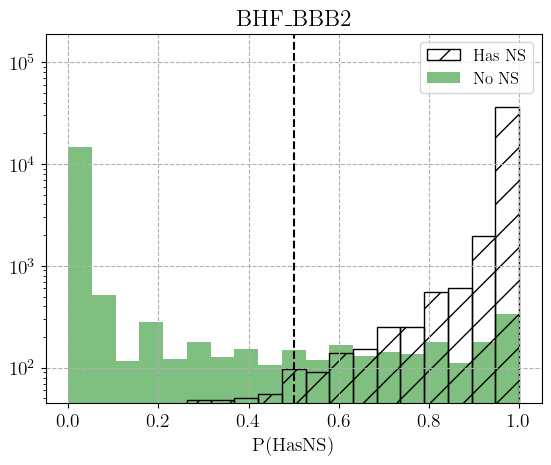
\includegraphics[width=0.45\textwidth]{/figs/KNN_BHF_BBB2_NShist.png}
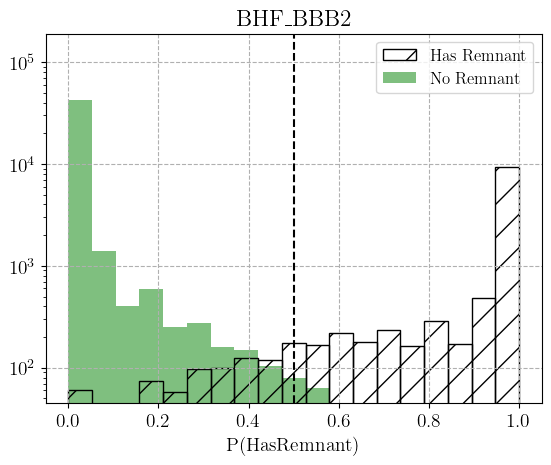
\includegraphics[width=0.45\textwidth]{/figs/KNN_BHF_BBB2_REMhist.png}
\caption{\label{fig:KNN_hist_BHFBBB2} Histograms BHF BBB2 KNN}
\end{figure}

\begin{figure}
\centering
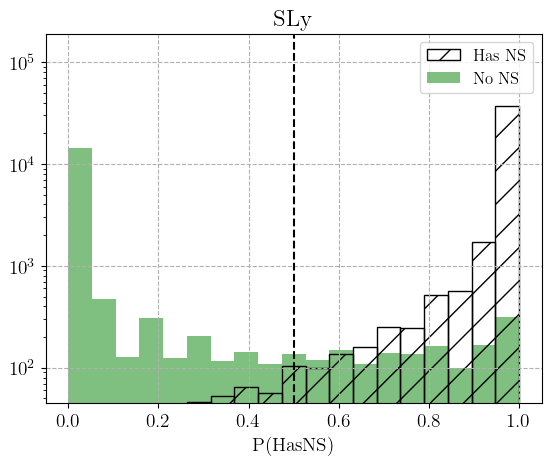
\includegraphics[width=0.45\textwidth]{/figs/KNN_SLy_NShist.png}
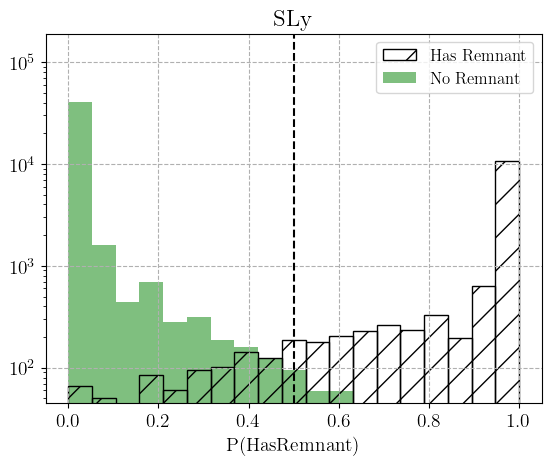
\includegraphics[width=0.45\textwidth]{/figs/KNN_SLy_REMhist.png}
\caption{\label{fig:KNN_hist_SLY} Histograms SLy KNN}
\end{figure}

\begin{figure}
\centering
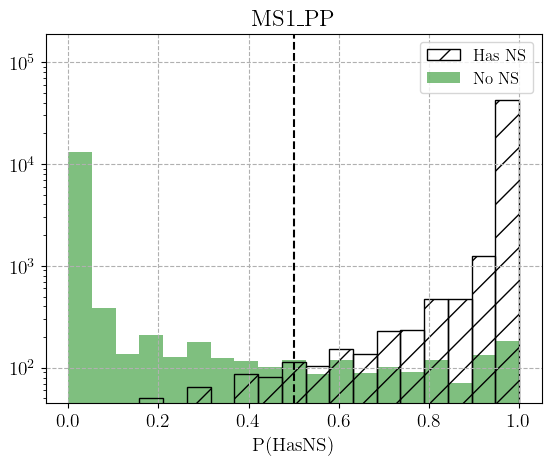
\includegraphics[width=0.45\textwidth]{/figs/KNN_MS1_PP_NShist.png}
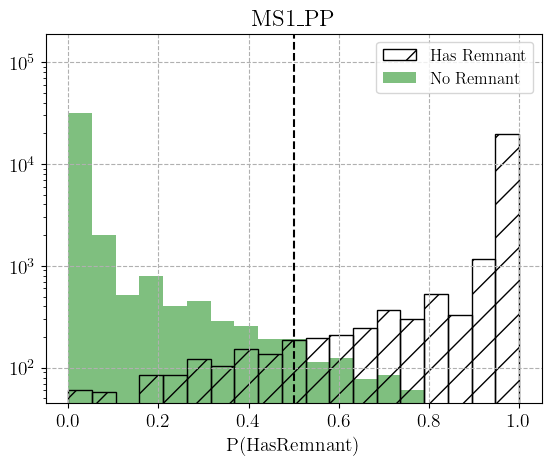
\includegraphics[width=0.45\textwidth]{/figs/KNN_MS1_PP_REMhist.png}
\caption{\label{fig:KNN_hist_MS1PP} Histograms MS1 PP KNN}
\end{figure}

Considering now the SLy EOS,  the model with these parameters gives a confusion matrix that is shown in Fig.~\ref{fig:KNN_confmat_SLY}.  The probability of having a NS as a function of $m_1$ and $m_2$  is shown in Fig.~\ref{fig:KNN_paramsweep_NS_SLY}. There are no big differences with different values of the spins, but the most remarkable one is that the model classifies better for 0-spin values, especially when $m_1$ is large.  There is also a dependence of the probability of having a remnant on the value of the spin that can be seen in Fig.~\ref{fig:KNN_paramsweep_REM_SLY}.This dependence is correct, since the probability of having a remnant increases for large values of $m_1$ at larger spin, but this dependence is given by the EOS. 

\begin{figure}
\centering
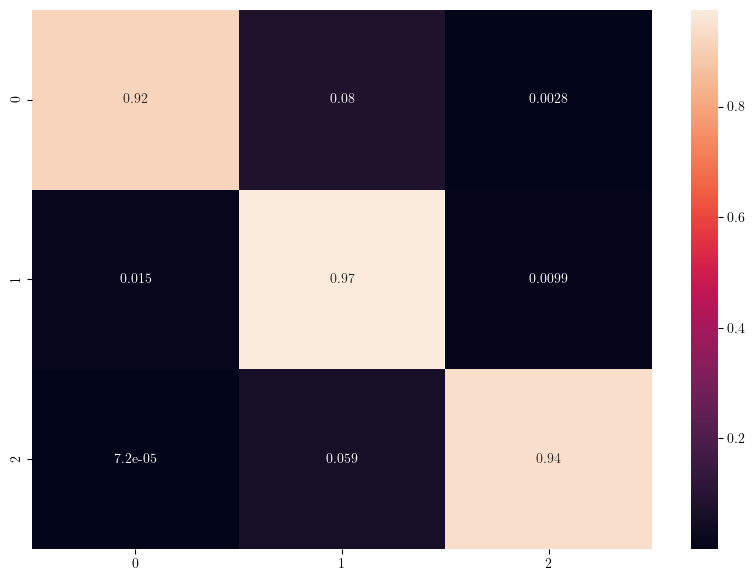
\includegraphics[width=0.45\textwidth]{/figs/KNN_confmat_SLy.png}
\caption{\label{fig:KNN_confmat_SLY} Confusion matrix SLy KNN}
\end{figure}

\begin{figure}
\centering
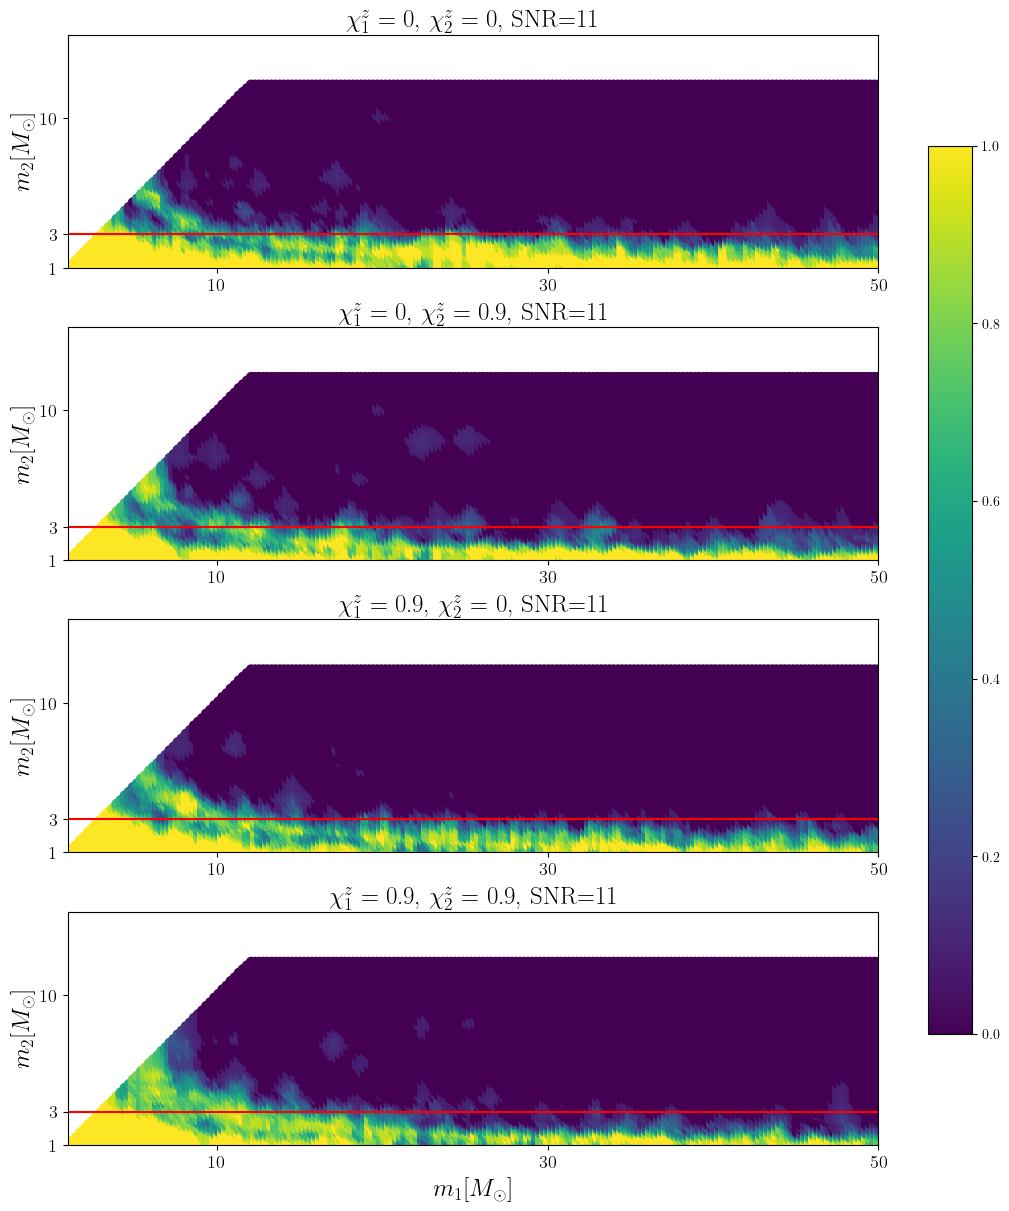
\includegraphics[width=0.45\textwidth]{/figs/KNN_param_sweep_spin_NS_SLy.png}
\caption{\label{fig:KNN_paramsweep_NS_SLY} Parameter sweep NS SLy KNN}
\end{figure}

\begin{figure}
\centering
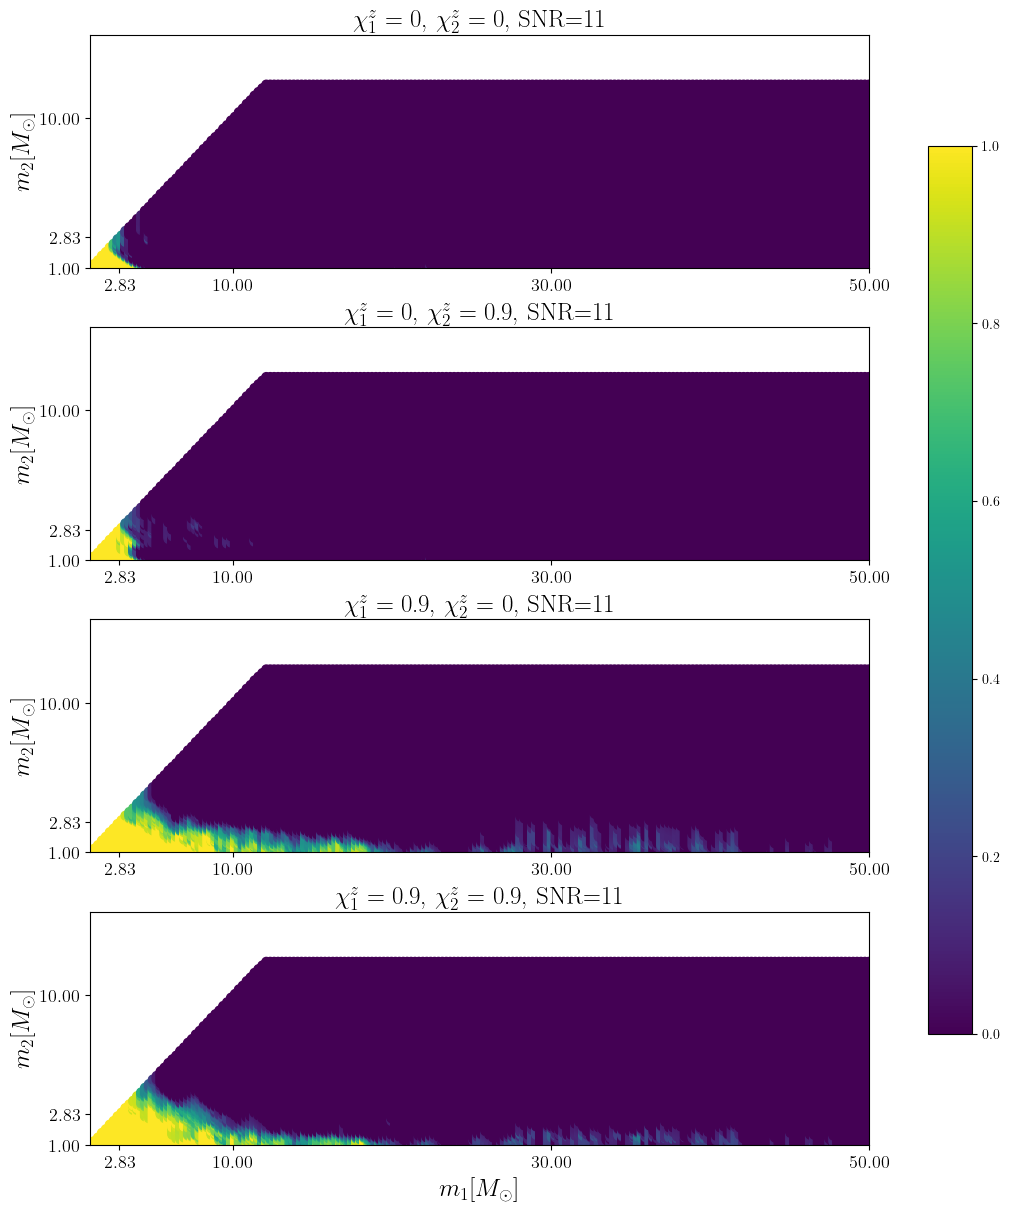
\includegraphics[width=0.45\textwidth]{/figs/KNN_param_sweep_spin_REM_SLy.png}
\caption{\label{fig:KNN_paramsweep_REM_SLY} Parameter sweep REM SLy KNN}
\end{figure}





In table \ref{tab:RFcross} we present a summary of best and second best hyperparameters found in the crossvalidation for each EoS, along the memory the model occupies and the difference in the score. As we can see, usually a forest with many trees has a second best option with far less that is lighter in memory and achieves a similar performance. The optimum maximum depth is always 15. Also the score achieved for every EoS is similar, and so we check that our accuracy is not NS model dependent.

\begin{table*}[h]
\centering
\begin{tabular}{@{}lcccccccc@{}}
\toprule
                                & \multicolumn{4}{c}{Best}                                & \multicolumn{4}{c}{Second best}                            \\ \midrule
\multicolumn{1}{|l|}{EOS}       & Trees & Depth & Size(MB)    & \multicolumn{1}{c|}{Score}      & Trees & Depth & Size(MB)    & \multicolumn{1}{c|}{$\Delta$score} \\ \midrule
\multicolumn{1}{|l|}{APR4\_BB}  & 300   & 15    & 94.7  & \multicolumn{1}{c|}{0.9683018}  & 50    & 15    & 15.7  & \multicolumn{1}{c|}{3.35e-5}       \\ \midrule
\multicolumn{1}{|l|}{BHF\_BBB2} & 80    & 15    & 24.4  & \multicolumn{1}{c|}{0.9685127}  & 300   & 15    & 91.6  & \multicolumn{1}{c|}{5.16e-5}       \\ \midrule
\multicolumn{1}{|l|}{H4}        & 80    & 15    & 29.6  & \multicolumn{1}{c|}{0.9618587}  & 300   & 15    & 111.4 & \multicolumn{1}{c|}{1.19e-4}       \\ \midrule
\multicolumn{1}{|l|}{HQC18}     & 300   & 15    & 93.7  & \multicolumn{1}{c|}{0.9673755}  & 100   & 15    & 31.3  & \multicolumn{1}{c|}{3.06e-4}       \\ \midrule
\multicolumn{1}{|l|}{KDE0V}     & 300   & 15    & 92.0  & \multicolumn{1}{c|}{0.9673295}  & 80    & 15    & 24.5  & \multicolumn{1}{c|}{2.06e-4}       \\ \midrule
\multicolumn{1}{|l|}{KDE0V1}    & 100   & 15    & 30.9  & \multicolumn{1}{c|}{0.96704954} & 80    & 15    & 24.5  & \multicolumn{1}{c|}{3.43e-5}       \\ \midrule
\multicolumn{1}{|l|}{MPA1}      & 80    & 15    & 27.2  & \multicolumn{1}{c|}{0.96601225} & 300   & 15    & 102.1 & \multicolumn{1}{c|}{8.19e-5}       \\ \midrule
\multicolumn{1}{|l|}{MS1\_PP}   & 300   & 15    & 113.5 & \multicolumn{1}{c|}{0.96563534} & 80    & 15    & 30.2  & \multicolumn{1}{c|}{1.15e-4}       \\ \midrule
\multicolumn{1}{|l|}{MS1B\_PP}  & 300   & 15    & 114.2 & \multicolumn{1}{c|}{0.96555340} & 100   & 15    & 38.0  & \multicolumn{1}{c|}{1.97e-4}       \\ \midrule
\multicolumn{1}{|l|}{RS}        & 300   & 15    & 103.8 & \multicolumn{1}{c|}{0.96447350} & 80    & 15    & 27.6  & \multicolumn{1}{c|}{2.36e-4}       \\ \midrule
\multicolumn{1}{|l|}{SK255}     & 300   & 15    & 105.8 & \multicolumn{1}{c|}{0.96472405} & 100   & 15    & 35.5  & \multicolumn{1}{c|}{3.69e-4}       \\ \midrule
\multicolumn{1}{|l|}{SK272}     & 300   & 15    & 109.0 & \multicolumn{1}{c|}{0.96401816} & 100   & 15    & 36.4  & \multicolumn{1}{c|}{1.99e-4}       \\ \midrule
\multicolumn{1}{|l|}{SKI2}      & 50    & 15    & 18.8  & \multicolumn{1}{c|}{0.96242338} & 300   & 15    & 112.8 & \multicolumn{1}{c|}{8.37e-5}       \\ \midrule
\multicolumn{1}{|l|}{SKI3}      & 50    & 15    & 19.0  & \multicolumn{1}{c|}{0.96174537} & 100   & 15    & 38.1  & \multicolumn{1}{c|}{6.62e-5}       \\ \midrule
\multicolumn{1}{|l|}{SKI4}      & 300   & 15    & 100.6 & \multicolumn{1}{c|}{0.96598969} & 30    & 15    & 9.8   & \multicolumn{1}{c|}{8.37e-5}       \\ \midrule
\multicolumn{1}{|l|}{SKI5}      & 100   & 15    & 38.2  & \multicolumn{1}{c|}{0.96343381} & 80    & 15    & 30.4  & \multicolumn{1}{c|}{1.16e-4}       \\ \midrule
\multicolumn{1}{|l|}{SKI6}      & 300   & 15    & 101.7 & \multicolumn{1}{c|}{0.96586928} & 30    & 15    & 10.0  & \multicolumn{1}{c|}{2.17e-4}       \\ \midrule
\multicolumn{1}{|l|}{SKMP}      & 300   & 15    & 100.2 & \multicolumn{1}{c|}{0.96544567} & 80    & 15    & 26.9  & \multicolumn{1}{c|}{1.69e-4}       \\ \midrule
\multicolumn{1}{|l|}{SKOP}      & 100   & 15    & 32.3  & \multicolumn{1}{c|}{0.96610459} & 300   & 15    & 96.2  & \multicolumn{1}{c|}{6.85e-5}       \\ \midrule
\multicolumn{1}{|l|}{SLy}       & 80    & 15    & 25.3  & \multicolumn{1}{c|}{0.96728884} & 300   & 15    & 95.2  & \multicolumn{1}{c|}{8.49e-5}       \\ \midrule
\multicolumn{1}{|l|}{SLY2}      & 100   & 15    & 31.8  & \multicolumn{1}{c|}{0.96745868} & 80    & 15    & 25.4  & \multicolumn{1}{c|}{2.38e-4}       \\ \midrule
\multicolumn{1}{|l|}{SLY9}      & 300   & 15    & 101.6 & \multicolumn{1}{c|}{0.96605993} & 100   & 15    & 34.1  & \multicolumn{1}{c|}{1.51e-4}       \\ \midrule
SLY230A                         & 300   & 15    & 95.5  & 0.96714915                      & 100   & 15    & 31.9  & 2.53e-4                            \\ \bottomrule
\end{tabular}
\caption{Comparison of the best and second best RF models obtained during crossvalidation for all EoS. We show the file size in MB of the forest, and the difference in score between the two options.}
\label{tab:RFcross}
\end{table*}

The ourperformance of HasREM against HasNS in RF is even more noticeable in the histograms in figures \ref{fig:RF_hist_BHFBBB2}, \ref{fig:RF_hist_SLY} and \ref{fig:RF_hist_MS1PP} for the highlighted EoS, where the bars of asigned probabilities do not intersect each other and therefore there exists a threshold value for perfect classification in the testing dataset.

\begin{figure}
\centering
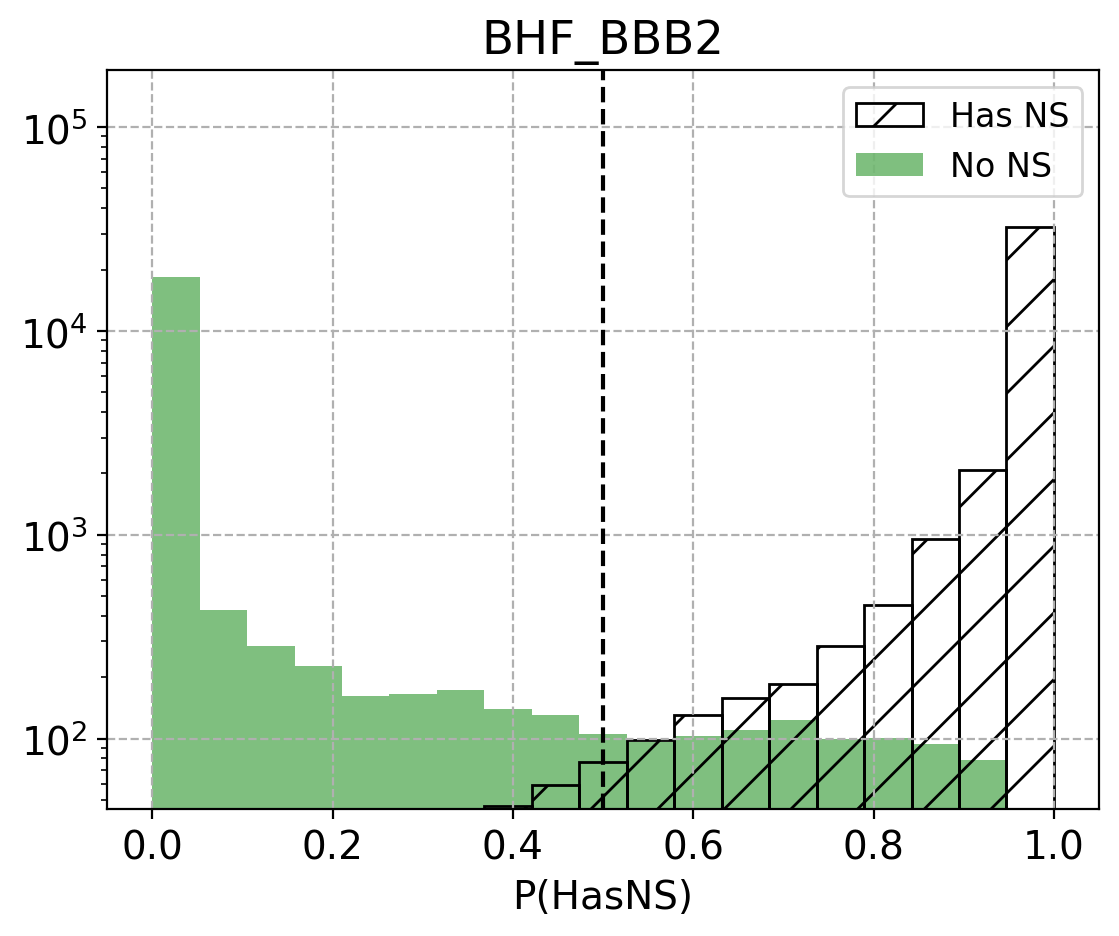
\includegraphics[width=0.45\textwidth]{/figs/BHF_BBB2_NShist}
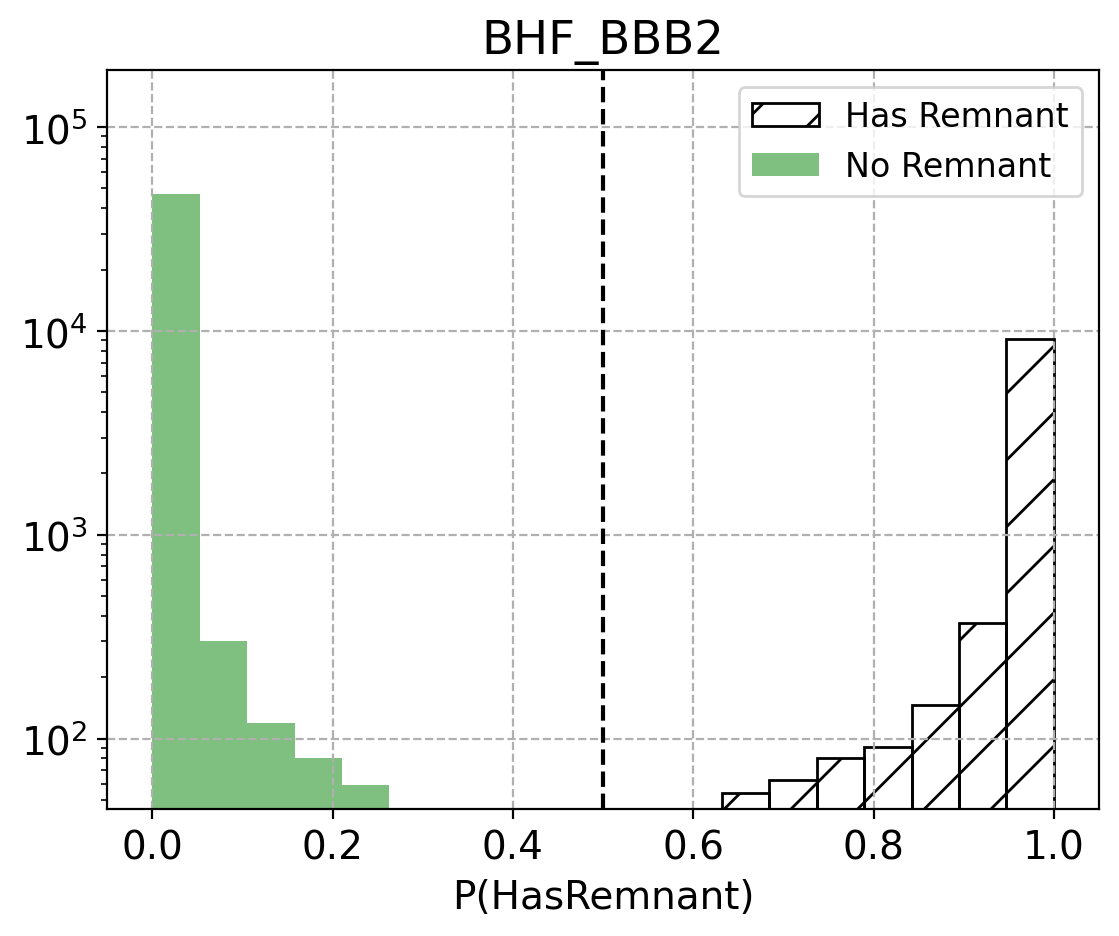
\includegraphics[width=0.45\textwidth]{/figs/BHF_BBB2_REMhist}
\caption{\label{fig:RF_hist_BHFBBB2} Histograms BHF BBB2}
\end{figure}

\begin{figure}
\centering
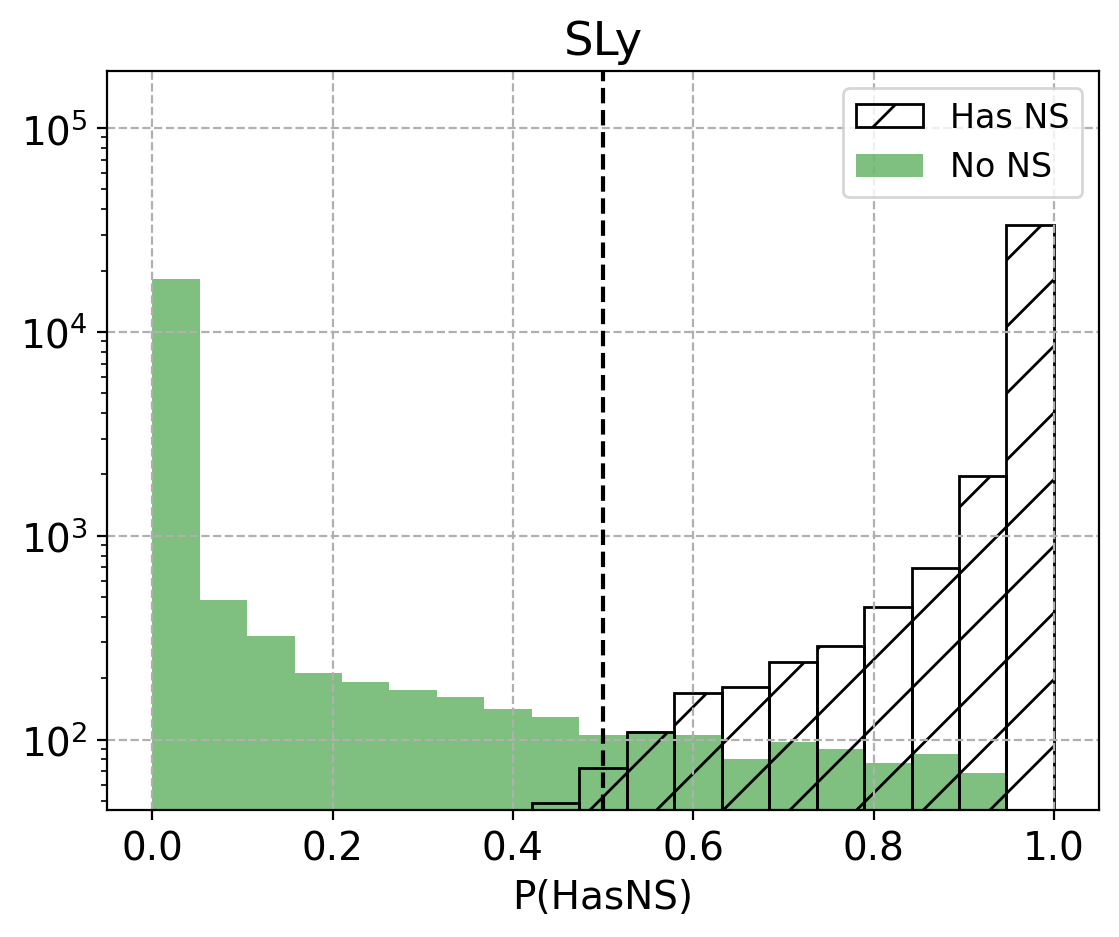
\includegraphics[width=0.45\textwidth]{/figs/SLy_NShist}
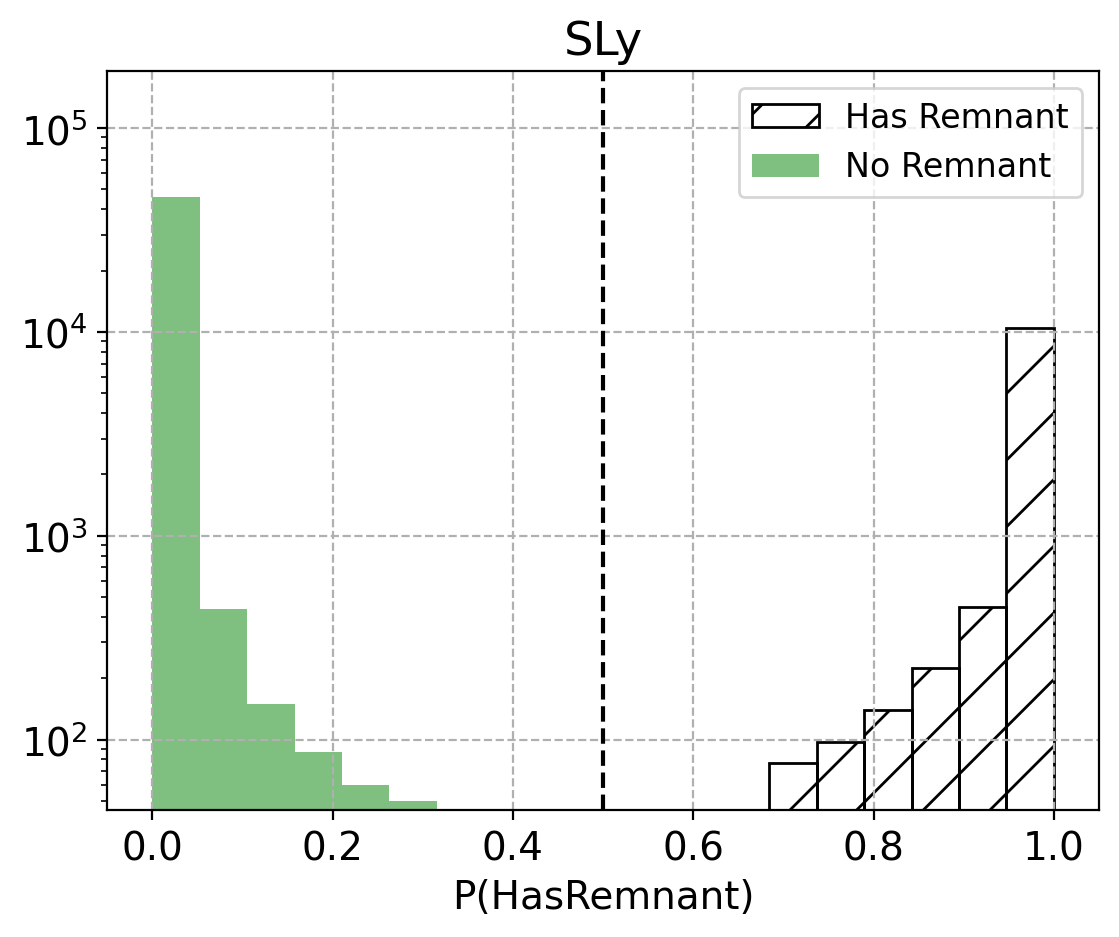
\includegraphics[width=0.45\textwidth]{/figs/SLy_REMhist}
\caption{\label{fig:RF_hist_SLY} Histograms SLy}
\end{figure}

\begin{figure}
\centering
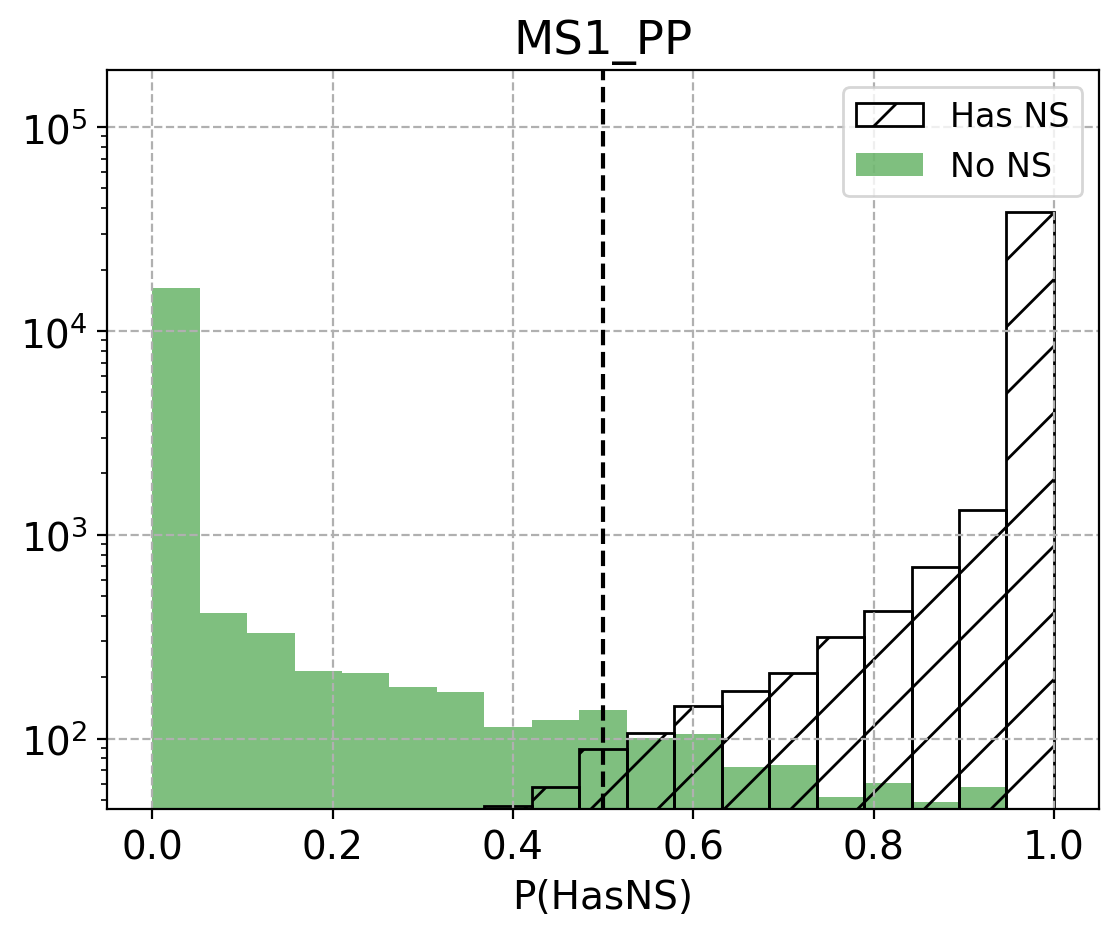
\includegraphics[width=0.45\textwidth]{/figs/MS1_PP_NShist}
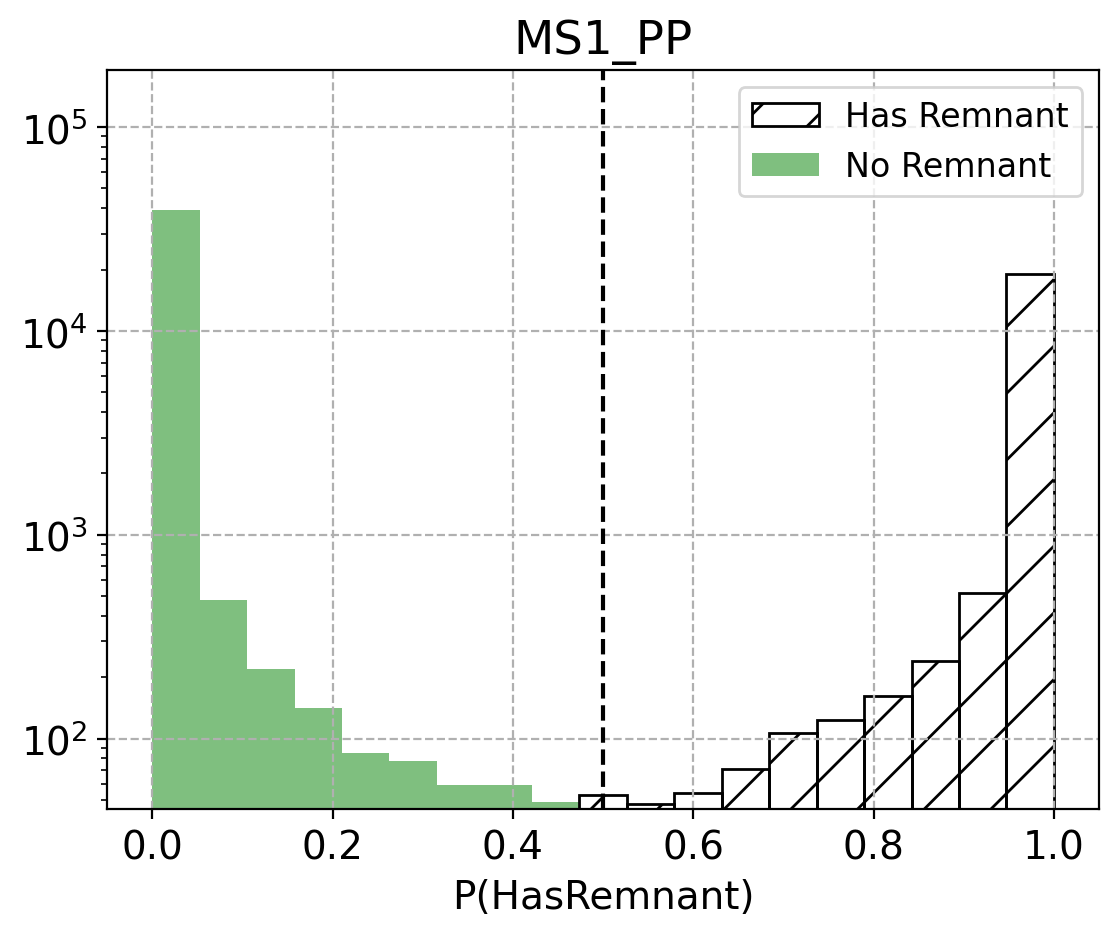
\includegraphics[width=0.45\textwidth]{/figs/MS1_PP_REMhist}
\caption{\label{fig:RF_hist_MS1PP} Histograms MS1 PP}
\end{figure}
